\chapter{Sequences and Series}
\label{chseqs}

We now start our study of functions, and how functions change and behave ``in the big
picture''. For this, we first consider functions on integers.

\section{Sequences}
\label{secsequences}

\begin{defn}
A \defini{sequence} is a function $a\colon N_0\to\R$, defined on the set $N_0=\{z\in Z\mid
z\ge 0\}$. If $i\in N_0$ and $a(i)$ is a value, we also call $i$ the \defini{index} or
the \defini{position} in the sequence.
Sometimes we ignore index $0$ and only consider sequences indexed by strictly positive
integers.
\end{defn}

The word ``index'' (plural: {\em indices})is the reason for denoting the argument by $i$ (and thus ultimately
the reason why ``i'' is the standard name for a loop variable when programming).

It often is convenient to write indices as subscript and to write $a_i$ in place of
$a(i)$. We will write $(a_i)$ to designate a sequence (that is the set of all values) in
contrast to a single value $a_i$.
\smallskip

Since sequences are a special case of functions, we can describe sequences in the same
way as functions. Often this is done by prescribing a rule, for example:
$a_i=i+1$ for the sequence
\[
a_0=1,\qquad a_1=2,\qquad a_2=3,\ldots
\]
Other examples would be the sequences $b_i=i^2+5$, $c_i [=\sum_{j=0}^i j]=${\em the sum
of the numbers from $1$ to $i$}, or $d_i=${\em the $i$-th prime number}.
\smallskip

With indices arranged easily as $1,2,3$, it also can be tempting to write a sequence by
giving its first few values, and expecting the reader to identify and continue the
pattern. For example
\begin{eqnarray*}
a_i&:&1,3,5,7,9,1,\ldots\\
b_i&:&10,9,8,7,\ldots\\
c_i&:&3, 3.1, 3.14, 3.141, 3.1415,\ldots
\end{eqnarray*}
While this seems convenient, guessing the right pattern can be difficult, and is
ambiguous. Indeed, despite its use in popular tests that ask the reader to identify the
rule for a given set of values, it is impossible to decide what the ``correct'' rule should
be. For example, consider the sequence
\[
2,4,6,8,10,\ldots
\]
which one might guess is given (assume we start indexing at $1$) by the rule $a_i=2i$
and has the next value $12$. But one can also argue that the next value is $-17$, based
on the rule
\[
a_i=-\frac{29}{120}x^{5}+\frac{29}{8}x^{4}-\frac{493}{24}x^{3}+\frac{435}{8}x^{2}
-\frac{3853}{60}x+29.
\]
Such problems therefore only make sense if we ask for the {\em simplest possible} answer
(however we might want to measure it), which immediately makes it a far more difficult
problem than we would want to consider here.
\medskip

As for functions, we also could consider plotting the values of a sequence, but since
they are only defined for integral arguments the result will be disconnected dots.

Finally, a sequence might be a sequence of data values (e.g. over time), which we know
in part and would like to predict in the future.

\section{Recursion}

Sequences are important in computer science, in that they can arise when indicating the
cost (that is number of calculation steps required) of an algorithm, for an input of a
given size $i$. In this context, sequences often are given through a \defini{recursion}.
That is, we give one (or several) initial values of the sequence, and then give a
formula how further values are determined from the previous ones. For example:
\[
a_1=3,\qquad a_i=a_{i-1}+2\mbox{\ for $i>1$}
\]
gives us the sequence $a_i=1+2i$, while
\[
s_1=1,\qquad s_i=s_{i-1}+i\mbox{\ for $i>1$}
\]
gives the sequence, whose $i$-th entry is the sum of integers from $1$ to $i$. It is
also possible to instead give values for new indices bigger than $i$, in the example
\[
s_{i+1}=s_i+(i+1).
\]

Recursions might refer to multiple prior values (and then one might need to define
multiple start values). The prototypical example of this is the \defini{Fibonacci
numbers}, defined as:
\[
f_0=0,\qquad f_1=1,\qquad f_{n+2}=f_{n+1}+f_n.
\]
We can determine arbitrary values $f_i$ by following through the recursion and evaluate
terms one by one. (This also shows that the values of the sequence are uniquely
determined.) Here for example:
\[
f_2=f_0+f_1=0+1=1,\quad
f_3=f_1+f_2=1+1=2,\quad
f_4=1+2=3,\quad
f_5=2+3=5,\ldots .
\]

\medskip

It still can be desirable, for a sequence given by a recursion, to determine a closed
(i.e. a direct value that requires no loop when evaluating)
formula for its values. Doing so, however often requires tools that are significantly
beyond this course (but see~\pointer{solvfibo}). Instead we shall illustrate how one can verify a closed formula for
a recursively defined sequence.
We do so with the above example of the ``sum of the first $i$ integers'' and the
recursion
$s_1=1$, and $s_i=s_{i-1}+i$. We claim that the formula $s_i=\frac{i(i+1)}{2}$ satisfies
the recursion. To show that this indeed is the case, we first check the base cases:
\[
s_i=\frac{1(1+1)}{2}=1.
\]
We then assume that the index is large enough for the recursive formula to hold (in this
example: $i>1$) and verify that the formula satisfies the recursion. That is
we evaluate the right hand side of the recursion when plugging in the formula:
\begin{eqnarray*}
s_{i-1}+i&=&\frac{(i-1)((i-1)+1)}{2}+i=\frac{(i-1)i}{2}+i\\
&=&\frac{i^2-i+2i}{2}=\frac{i^2+i}{2}=\frac{i(i+1)}{2}
\end{eqnarray*}
and compare with the formula for the left hand side $s_i=\frac{i(i+1)}{2}$. (One could
analogously use the alternative recursion formula $s_{i+1}=s_i+(i+1)$ instead, and then
would have to simplify the left hand side when evaluating
$s_{i+1}=\frac{(i+1)(i+1+1)}{2}$.)

%
%\[
%f_n
%=\frac{1}{\sqrt{5}}\left(\left(\frac{1+\sqrt{5}}{2}\right)^{n}-\left(\frac{1-\sqrt{5}}{2}\right)^{n}\right).
%\]

\subsection{Application: estimating the cost of a program}

%BN edit AH
An important application of sequences and recursion is in estimating the
number of steps a recursive algorithm will take to completion. Here the
sequence value at position $i$ is defined to be the number (or a bound
thereof) of steps taken by the algorithm for an input of size $n$. 

Consider, for example, the following (very naive) insertion-sort algorithm. 
To sort a list $L$ consisting of $n$ numbers, we first sort (by a recursive
call) the first $n-1$
numbers and then insert the $n$-th element in the right position in the list.
\begin{verbatim}
define: sort(L,n)
input: L, a list of integers, to be sorted
        n, up to which position to sort
procedure:
if (n > 1) then # Otherwise no need to sort
  sort(L,n-1); # recursively sort the first n-1 elements
  a:=L[n];
  p:=1; # find position of first entry larger than a
  while p<n and L[p]<=a do 
    p:=p+1;
  od;
  for j from n-1 downto p do # shift entries up
    L[j+1]:=L[j];            # to make space at p
  od;
  L[p]:=a;
fi;
\end{verbatim}

% Tried writing a more explicit algorithm but felt like it was too complicated
% to communicate the point - hopefully this  gets the idea across without
% being too handwavy.

For example, if $L = [5,13,12]$, how does \verb+sort(L,3)+ get processed? 
We call \verb+sort(L,2)+, which in turn calls
\verb+sort(L,1)+, which does nothing. Exiting back to $n=2$ we set $a=L[2]=13$ and (since
$L[1]=5<13$) get $p=2$, keeping $13$ in the second position.
Exiting the recursion and getting back to $n=3$, we find (again) that $p=2$, and
shift the 13 into position 3, inserting 12 into position 2.
\smallskip

We want to know how many comparisons of elements our algorithm might have to
do. (Such comparisons only happen in the \texttt{while} loop condition.) For
this, we define a sequence $\text{cost}_n$, that is an upper bound on the
number of comparisons required by this algorithm to sort a list of length
$n$.

Recall that a recursive formula for a sequence is given by a collection of initial values
and a formula which determines the value of the sequence at $n$ based on previous
terms of the sequence.
Our initial value will be $\text{cost}_1$. This is the number of comparisons
needed to sort a list of length one, which is 0, since we have nothing to
check. Thus $\text{cost}_1 = 0$.

For $n>1$, the algorithm calls itself recursively for length $n-1$ (at cost
$\text{cost}_{n-1}$, and then compares the last element $a$ to potentially
all\footnote{The clever reader might already think on how to improve the
algorithm by using {\em binary search} to find the correct position in fewer
steps.} $n-1$ elements in the list. The cost thus satisfies the recursion
\[
\text{cost}_n = \text{cost}_{n-1} + (n-1).
\]
For example, $\text{cost}_2 = \text{cost}_1+1=0+1=1$ and $\text{cost}_3 =
\text{cost}_2+2=1+2=3$.

By `peeling' back the layers of the recursion, we could get a formula (this
is a little bit beyond the expectations for this course) for
$\text{cost}_n$ as:
\begin{align*}
\text{cost}_n &=  \text{cost}_{n-1} + (n-1) \\
&=  \text{cost}_{n-2} +(n-2) + (n-1) \\
& =  \text{cost}_{n-3} + (n-3) +(n-2)+(n-1) \\
&=\ldots \\
&= 1 + 2 + \ldots + (n-3) + (n-2) + (n-1) \\
&= \sum_{k=1}^{n-1} k \\
&= \frac{n(n-1)}{2}.
\end{align*}

In any case, (even without the arithmetic done in the previous paragraph),
the reader should be able to use the same tools as above to verify that the
recusion
\[
\text{cost}_1=0; \text{cost}_n = \text{cost}_{n-1} + (n-1).
\]
is satisfied by the formula
\[
\text{cost}_n = \frac{n(n-1)}{2}.
\]
We have thus {\em proven} that the (not very good) algorithm given has a worst
case requirement of $\frac{n(n-1)}{2}$ comparisons to sort a list of length
$n$.

%It is important to note that the base case of the recursion for $\text{cost}_n$
%depends on the implementation of the given pseudocode for $sort(L,n)$.
%If the program were to perform some sort of trivial check when the list is
%of length 1, then $\text{cost}_1 = 1$ and
%the cost function would be given as
%	\[
%	\text{cost}_n = \frac{n(n+1)}{2}.
%	\]
%Worrying about such small details is cumbersome, so computer scientists prefer
%to think about cost functions in terms of complexity classes, a concept covered
%later in the text. For now we will write $\text{cost}_n = \mathcal{O}(n^2)$ to
%mean that the cost function grows similarly to $n^2$.

\section{Monotonous and Bounded Sequences}

We are interested in investigating the long-term (that is, values for large indices)
behavior of sequences. For this we define the following properties:
\begin{defn}
Let $(a_i)$ be a sequence. Then this sequence is
\begin{description}
\item[\defini{monotonically increasing}], if $a_{i+1}\ge a_i$ for all $i$.
\item[\defini{strictly monotonically increasing}], if $a_{i+1}> a_i$ (and $a_{i+1}\not=a_i$) for all $i$.
\item[\defini{bounded from above}], if there exists a number $B\in\R$, such that $a_i\le B$ for all $i$.
\end{description}
We define \defini{monotonically decreasing}, \defini{strictly monotonically decreasing},
and \defini{bounded from below} in the obvious way by reverting the inequalities.
\end{defn}

For example, consider the sequences
\begin{eqnarray*}
a_i&=&5-\frac{1}{i},\\
b_i&=&5+i,\\
c_i&=&5+(-1)^i.\\
\end{eqnarray*}
Then the sequences $(a_i)$ and $(b_i)$ are (strictly) monotonically increasing, since
\[
a_{i+1}=5-\frac{1}{i+1}\ge 5-\frac{1}{i}=a_i
\mbox{\ and \ }
b_{i+1}=5+(i+1)\ge 5+i=b_i.
\]
The sequence $(c_i)$ is not monotonically increasing, as 
\[
c_2=5+(-1)^2=6\not\le 4=5+(-1)^3=c_3.
\]Similarly, we have that $(a_i)$ and $(c_i)$ are both bounded from above, since we have
that $a_i\le 10$, $c_i\le 10$ for all $i$ (i.e. we can set $B=10$).
Note that we do not need to pick the bound as tight as possible. (It is a separate
question of what a tighter possible bound is, but we shall not investigate that.)

The sequence $(b_i)$ is not bounded from above. Suppose that $B\in\R$ was a bound and
let $i=\lceil B\rceil$ the smallest integer not smaller than $B$ (i.e. we round up).
Then $i\ge B$ and thus
\[
b_i=5+i\ge5+B>B,
\]
in contradiction to the assumption that $B$ is an upper bound.

All three sequences $(a_i)$, $(b_i)$, $(c_i)$ are bounded from below (e.g. by $1$).
However it is possible that a sequence is neither monotonous, nor bounded; for example 
$d_i=5+(-1)^i\cdot i$.

\section{Convergence}
\label{seclimits}

The best case for describing the long-term behavior of a sequence is if
its values ``settle down'' as the index increases. As with a ball rolling in a bowl, this
might not mean to stand still, but simply getting
closer and closer to some value $L$ (which we shall call the limit of the sequence).
Such a number must be unique, if it exists.
In this case we call the sequence \defini{convergent} (otherwise:
\defini{divergent})
and $L$ the \defini{limit} of the
sequence and write $L=\lim\limits_{i\to\infty}a_i$. (We will give a more formal
definition below.)

In the examples of the last section, this should be the case for the sequence $\{a_i\}$
which gets closer and closer to $5$, while the sequence $\{b_i\} $and $\{d_i\} $``run
away'' and $\{c_i\}$ jumps around but never settles down.

\subsection{Finding limits}

Since sequences get close to the limit, one way one can attempt to determine a limit
(and whether a sequence converges) is by evaluating the sequence for large values of the
index and to see whether the values seem to converge. This of course is not a proof
(since we do not know whether we have chosen large enough indices), but it often gives a
good idea in practice.

For sequences given by quotients of polynomials -- say
\[
a_i=\frac{6i^5+i^2-i-1}{5i^5-8i^2+i+1}
\]
there actually is a rule (we will see it later in~\pointer{seclhopital}):
\begin{itemize}
\item If the degree of the denominator is larger than the degree of the numerator, the
sequence converges to zero.
\item If the degree of the denominator is smaller than the degree of the numerator, the
sequence values will get arbitrary large in absolute value, the sequence does not
converge (or converges to $\pm\infty$).
\item If the degree of numerator and denominator are equal, the sequence converges to
the quotient of the leading coefficients -- in the example $6/5$.
\end{itemize}

We also note (without proof) that limits behave reasonably with respect to arithmetic:
\begin{lemma}
\label{limitlaws}
Let $\{a_i\}$, $\{b_i\}$ be sequences such that
$\lim\limits_{i\to\infty} a_i=A$,
$\lim\limits_{i\to\infty} b_i=B$. Then
\begin{itemize}
\item $\lim\limits_{i\to\infty} (a_i+b_i)=A+B$.
\item $\lim\limits_{i\to\infty} (a_i-b_i)=A-B$.
\item $\lim\limits_{i\to\infty} (a_i\cdot b_i)=A\cdot B$.
\item If $B\not=0$ then $\lim\limits_{i\to\infty} (a_i/b_i)=A/B$.
\end{itemize}
\end{lemma}

We also note that while it can be useful to talk about a limit infinity (say for the
sequence $a_i=i$), but these limit laws do not necessarily apply to such a situation.

\subsection{Proving Limits}

Our next task is to give a formal criterion for convergence. After all, it is not good
enough to simply say ``I know it if I see it''. This criterion, as we will use it, might
seem somewhat complicated, but ultimately evolved (over decades of failed attempts in the
19th century) as being unambiguous and formally testable. 

This definition also will serve as a model for the formalization of concepts in calculus.
\medskip

The basic idea is that we want to be able to corral-in the terms of the sequence at some
time, and then can (again at a suitable point in time) make that corral smaller (without
moving it around), and
smaller again, to become arbitrary small (and not become larger again).
In other words: If someone tells us how small the corral should be, we must be able to
point to a time (that is: to an index!) from when on the corral will be that small.

Formally, what we just called a corral, will be the set of numbers around (at a given
distance) a fixed,
unmovable point $L$, which we will call the \defini{limit} of the sequence -- the number
that the sequence converges towards.

Traditionally, mathematicians use the Greek letter ``epsilon'' ($\varepsilon$)
to denote the distance,
and our corral thus is the set
\[
\{a\in\R\mid \sz{a-L}\le\varepsilon\}
\]
We thus have established criterion for convergence:
\begin{itemize}
\item There is a number $L$ so that
\item Given an (arbitrary small) corral size $\varepsilon$
\item We can find an index (we shall call $N$. This $N$ will depend on $\varepsilon$)
\item from when on (i.e. for $i\ge N$) all entries $a_i$ of the sequence will be
at most $\varepsilon$ away from $L$.
\end{itemize}
Or, more formally:
\begin{defn}
A sequence $\{a_i\}$ \defini{converges}, if there exists a number $L$,
such that for an arbitrary $\varepsilon>0$ we can find
an $N$ such that $\sz{a_i-L}\le\varepsilon$ once $i\ge N$. In symbols:
\[
\forall\varepsilon>0\exists N:\forall i\ge N: \sz{a_i-L}\le\varepsilon.
\]

We write $L=\lim\limits_{i\to\infty} a_i$ and call it the
\defini{limit} of the sequence.
\end{defn}
\begin{note}
Some books write the inequalities strictly ($i>N$ etc.). This will not
change the property, since the statement is for all $\varepsilon$.
\end{note}

\begin{figure}[t]
\begin{center}
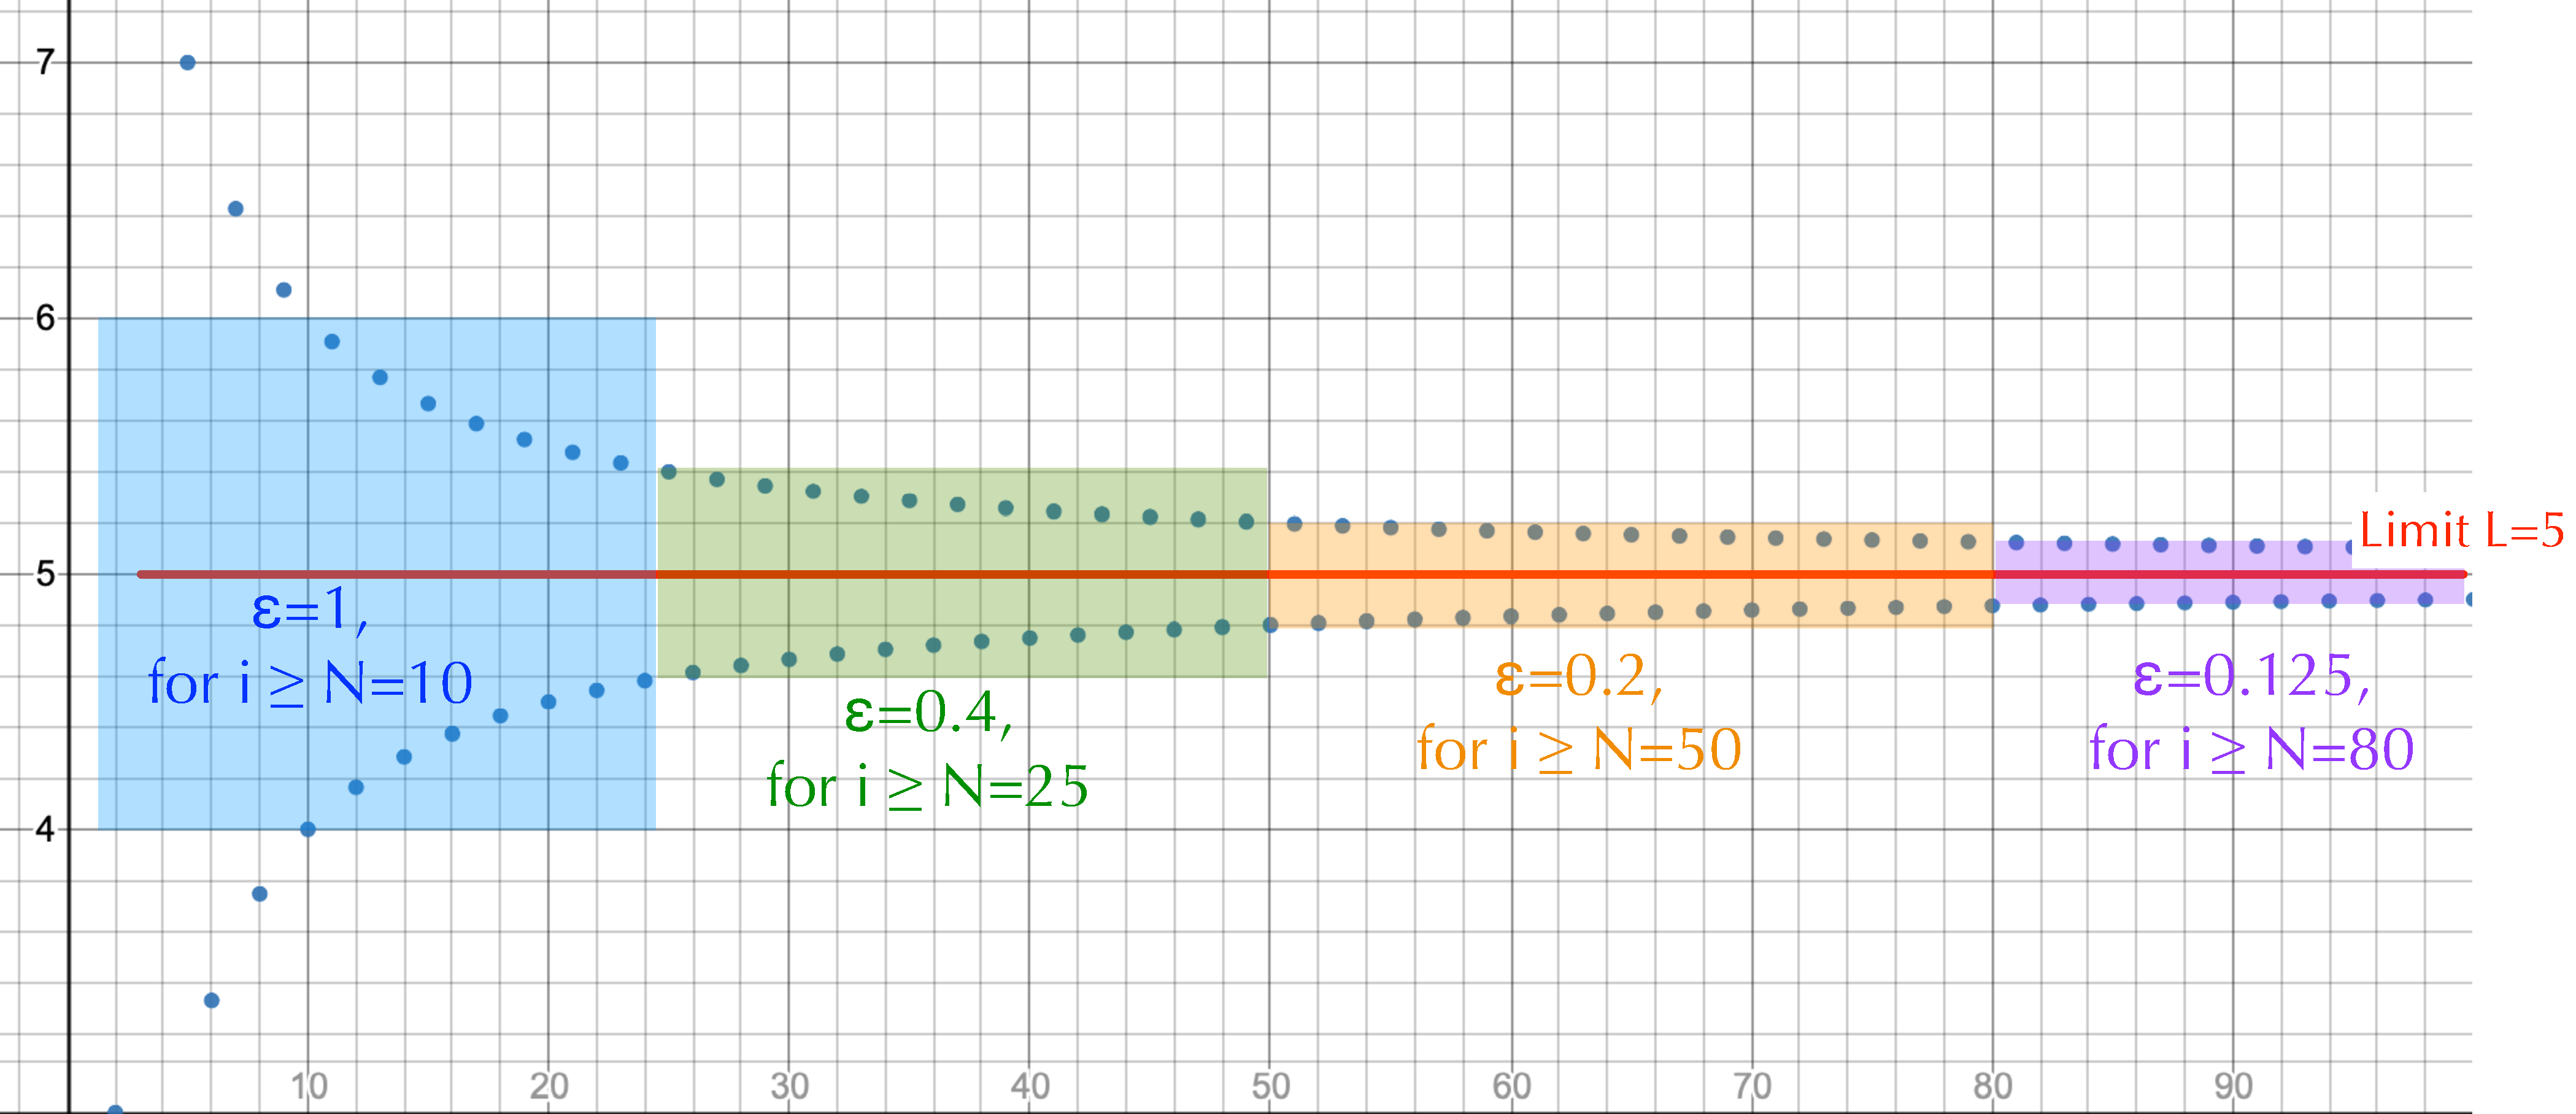
\includegraphics[width=12cm]{pic/LimitCorral.pdf}
\end{center}
\caption{A convergent sequence $a_i=5-(-1)^i\frac{10}{i}$}
\label{figlimitcorral}
\end{figure}

For example, consider the sequence given by 
$a_i=5-(-1)^i\frac{10}{i}$, depicted in Figure~\ref{figlimitcorral}. We set
$L=5$ and choose $\varepsilon=1$. Then for $N=10$ we have
that $\sz{a_i-L}\le\varepsilon$ when $i\ge N$. Similarly, we
determine the corresponding $N$-values for $\varepsilon=0.4$,
$\varepsilon=0.2$, and $\varepsilon=0.125$.

The condition however requires this statement to hold for {\em any
arbitrary} $\varepsilon>0$, not just for the four values we illustrated. We
thus need to give a general proof for an arbitrary $\varepsilon$. For that,
we start with a scratch calculation to find when $\sz{a_i-L}<\varepsilon$
and solve for $i$:
\[
\varepsilon\ge \sz{a_i-L}=\sz{5-(-1)^i\frac{10}{i}-g}=\sz{-(-1)^i\frac{10}{i}}=
\frac{10}{i}
\]
Since $i$ and $\varepsilon$ are both positive, we can multiply by $i$ and
divide by $\varepsilon$ and get
\[
i\ge\frac{10}{\varepsilon}.
\]
The right hand side is the value we chose for $N$ in the actual proof that
uses the work of this scratch calculation:

\begin{quote}
\underline{Let $\varepsilon>0$ and set} $N=\frac{10}{\varepsilon}$.
\underline{Then, for $i\ge N$ we have that}
\begin{eqnarray*}
\sz{a_i-L}&=&\sz{5-(-1)^i\frac{10}{i}-g}=\sz{-(-1)^i\frac{10}{i}}=
\frac{10}{i}\\
&\le&\frac{10}{N}=\frac{10}{10/\varepsilon}=\varepsilon.
\end{eqnarray*}
\underline{and thus $\{a_i\}$ converges to $L$.}
\end{quote}

With the scratch calculation beforehand, and the choice of $L$, it is of
course pre-determined that we will get $\sz{a_i-L}\le\varepsilon$. The
argument just presents the result of the scratch calculation in a format
corresponding to the definition of convergence.

Note that some of the text in the proof was underlined. This text will
essentially be always the same in any proof for convergence of a sequence,
while the remainder is basically built from the scratch calculation.

\begin{note}
\label{cauchycrit}
You might find this criterion for convergence somewhat unsatisfactory, in that it requires
the limit $L$ to be given. Is is clear that we can always calculate, or represent this
limit exactly? Consider for example the recursive sequence, defined by
\[
a_1=1,\qquad a_{i+1}=1+\frac{1}{a_i}.
\]
If we write a program to calculate values $a_i$ for increasingly large indices, we find that
the sequence seems to converge to a number $1.618033988749894848\ldots$. But what is
this limit\footnote{In this case, one can actually calculate it as a solution to the
quadratic equation $x=1+1/x$}, how can we express it and use it in a limit proof? 
To work around such problems, mathematicians often use a somewhat different criterion,
called the~\defini{Cauchy criterion} 
(see Wikipedia), that uses not the distance from sequence values to
the limit, but of sequence values never straying too far apart from each other. It
however is a bit more complicated to work with, which is the reason for the choice of
a more basic criterion here.
\end{note}

The reason for looking at formal proofs is that this is a prototype for the way formal
proofs work in Calculus\footnote{When doing proofs, the topic is often called
``Analysis''}. One argues about differences, typically denoted by $\varepsilon$ or its
causing $\delta$, becoming arbitrary small, but still being nonzero.

\section{Limits, Bounds and the Real numbers}

IF a sequence converges, its values cannot become arbitrary large, since at some point
they need to start getting close to the limit. This implies that a convergent sequence
must be bounded.
On the other hand, being bounded does not make a sequence
convergent, as the example $(-1)^i$ shows.

Things however become interesting if a sequence is monotonous and bounded (that is
increasing and bounded from above, or decreasing and bounded from below). We have the
following theorem:
\begin{thm}
Every monotonically increasing sequence that is bounded from above must converge to a
limit $L\in\R$. (As must every decreasing sequence bounded from below.)
\end{thm}
Conceptually this seems clear -- if we can never go back, nor cross a line, we eventually
must become stationary. A formal proof however is far beyond the scope of this course.

Note that the limit in such a case is not necessarily the bound used, but it is the
``best possible'' bound (formally called the \defini{suprenum}).
\medskip

This statement might seem more of a curiosity and have little relevance for
computational sciences. The reason we mention this fact is in that it ultimately gives a
justification for and explanation of what the real numbers are. So far, we defined
them, somewhat sloppily, as the $x$-coordinates of all points on the number line, or as
numbers with infinite decimal expansions. But that is 
only half the truth. Formally:

\begin{quote}
The real numbers are the limits of bounded, monotonous sequences.
\end{quote}

This construction is also the reason for why we use the real numbers (and not just
rational numbers of arbitrary large denominator and arbitrarily good expansions): They
are required to get limits of sequences that should converge. Such limits do not
necessarily exist in the rational numbers -- take for example the sequence recursively
defined in Note~\ref{cauchycrit}, whose limit is the irrational number
$\frac{1+\sqrt{5}}{2}$.
(There is a formal construction of the real numbers that defines an equivalence
relation on sequences -- multiple sequences might have the same limit -- and defines
the real numbers as equivalence classes of sequences under this relation.)

But the real numbers do not only numbers involving roots. Actually there are infinitely
(in an overwhelming sense) more real numbers, than numbers that can be expressed as
roots of polynomials. (Such numbers are called \defini{transcendental}.) You will have
seen some examples in school: $\pi$, $e$. But these numbers are like dark matter. While
they are overly abundant and around everywhere, it is hard to get hold of them (as one
would have to give a sequence that has them as limit).
\smallskip

Of course anything we can measure in the real world, anything we can represent as number
on the computer, is a rational number. The reason we use the real numbers is so that
limits exist!

\section{Series}

A series is a special sequence, in which we sum up the terms of another
sequence, that is it is the sequence of \defini{partial sums}.  If the
sequence we are summing over is $a_i$, we have the $i$-th partial sum as
\[
p_i=a_0+a+1+a_2+\cdots+a_{i-1}+a_i=\sum_{j=0}^i a_j,
\]
where the $\sum$ notation is basically a mathematician's version of a for-loop.
(Note that we need to use a different variable for the loop than for the loop end.)

If this sequence of partial sums converges we write the limit as an infinite sum.
\[
\sum_{j=0}^\infty a_i=\lim_{i\to\infty} p_i=\lim_{i\to\infty} \sum_{j=0}^i a_j.
\]
For example, we could sum over the
sequence $a_i=1/2^i$ and get the sequence of partial sums:
\[
p_0=1,
p_1=1+\frac{1}{2}=\frac{3}{2}, 
p_2=1+\frac{1}{2}+\frac{1}{4}=\frac{7}{4}, \ldots
\]
Here, it is not hard to see that the partial sums are
\[
p_i=\frac{2^{i+1}-1}{2^i}
\]
and this sequence thus has the limit
\[
\sum_{i=0}^\infty \frac{1}{2^i}=2,
\]
that is the infinite summation yields a finite number.
\smallskip

Clearly, the sequence over which we are summing must go to zero for the series to
converge. But that is not sufficient. For example, one can show that the series
\[
\sum_{i=1}^\infty \frac{1}{i}
\]
(called the \defini{harmonic series}) will not converge but go to infinity.

As an interesting aside, the program
\begin{verbatim}
s=0
old=-1
i=1
while s>old :
    old=s
    print(i, ": ",s)
    i=i+1
\end{verbatim}
%    s=round(s+1/i,6)
(which calculates the partial sums $\sum_{i=1}^n \frac{1}{i}$ for increasing
values of $n$ and terminates when they stop increasing) will
actually terminate (due to rounding errors) after a long time and thus
make it look as if the the series converges. But it does not!
\medskip

There are a number of criteria and tests to see whether a particular series converges,
and you will find examples and applications in any Engineering Calculus book. In this
course however we are not investigating this question, but will look at two particular
kinds of series (where it is relatively easy to indicate convergence).

\begin{note}
There is some subtlety with infinite summations: Usually we have that $a+b=b+a$, but it
is possible that a series changes its value (i.e. the limit of the partial sums), or
even whether it converges, if we change the order of summation.
This cannot happen if the sequence converges and all terms are positive -- the issue is
basically that we can unbalance positive and negative terms by moving some more and more
towards infinity.
\end{note}

\section{Geometric Series}

A sequence is called \defini{geometric} if its terms grow by a constant
factor $r$, that is, if the starting term
is $a$, the sequence is 
\[
a, ar, ar^2, ar^3, ar^4,\ldots
\]
We will assume that $r\not=1$, as the sequence is otherwise boring.

%As a second example of geometric growth we consider university
%scholarships which come from endowments.  In this case, an endowment (a
%fixed sum)
%is given to the university. A scholarship then is funded from the interest
%of this money (without using up the money, the scholarship therefore exists
%forever).
%
%\begin{Example}[Endowments]
%Delighted by the calculus course he took at CSU, an alumnus wants to endow a
%scholarship for mathematics students that will pay {\$}$2000$ each year. The
%university guarantees an interest rate of $5$\% per year.
%How much must the alumnus donate to guarantee this
%scholarship will be available forever?
%
%\solution
%If we let $x$=the value of the endowment, then after one year the
%endowment is worth $1.05 \cdot x$ and we want to give a {\$}$2000$
%scholarship, so we want $1.05x=x+2000$.  Therefore the endowment
%will never be touched and the scholarship is funded by the interest
%earned.  Solving this equation we get $0.05x=2000$ which gives us
%that $x=40,000$.  Therefore the alumni must give an endowment of
%{\$}$40,000$ to guarantee the scholarship is funded forever.
%\end{Example}
%\medskip

A geometric series now is a series whose terms show geometric growth, i.e.
$a_i=r\cdot a_{i-1}$ for a constant $r$, independent of $i$.
This type of series has applications in several fields
including physics, biology, economics and finance.
%We will look at a
%few examples of where geometric series occur in our everyday lives,
%including repeating decimals and calculating dosage of medicine.

\begin{defn}
Let $r$ be a ratio and $a$ any nonzero constant. A \defini{geometric series}
is a series of the form
\[
a+ ar + ar^{2}+ \ldots + ar^{n-1}+ \ldots = \sum_{n=1}^{\infty}
ar^{n-1} =a\sum_{n=1}^\infty r^{n-1}=a\sum_{n=0}^\infty r^n
\]
The $k^{th}$ partial sum $p_{k}$ of a Geometric series
$\displaystyle{\sum_{n=0}^{\infty} ar^{n}}$ is the (finite) sum of
the first $k+1$ terms:
\[
p_{k} = a + ar + ar^{2} + \ldots + ar^k =
\sum_{i=0}^k ar^{i}
\]
\end{defn}

A simple example of geometric growth is something that grows by a factor
each time unit. Suppose that a museum starts with
$a=100$ visitors per year and each year increases its visitor numbers by
$3\%$. That is the visitor number after $i$ years is $100\cdot 1.03^i=a\cdot
r^i$ for $r=1.03$. 
If we ask for the total number of visitors after $n$ years we get:
\[
\sum_{i=0}^n a\cdot r^i.
\]

%As an example of a geometric series we look at the ``Race course paradox'' of
%Zeno\footnote{Zeno of Elea, Greek philosopher, ca. 490 BC - ca. 430 BC}.
%Suppose a runner wanted to travel a given distance, say one kilometer. Then
%he must first travel the first half kilometer, and the next half kilometer
%remains.  Next the runner must travel half of the next half kilometer -- a
%quarter kilometer  -- and the next quarter kilometer remains. It might seem
%(so claimed Zeno) as if the runner never reaches the goal.
%
%\begin{figure}[h]
%\begin{center}
%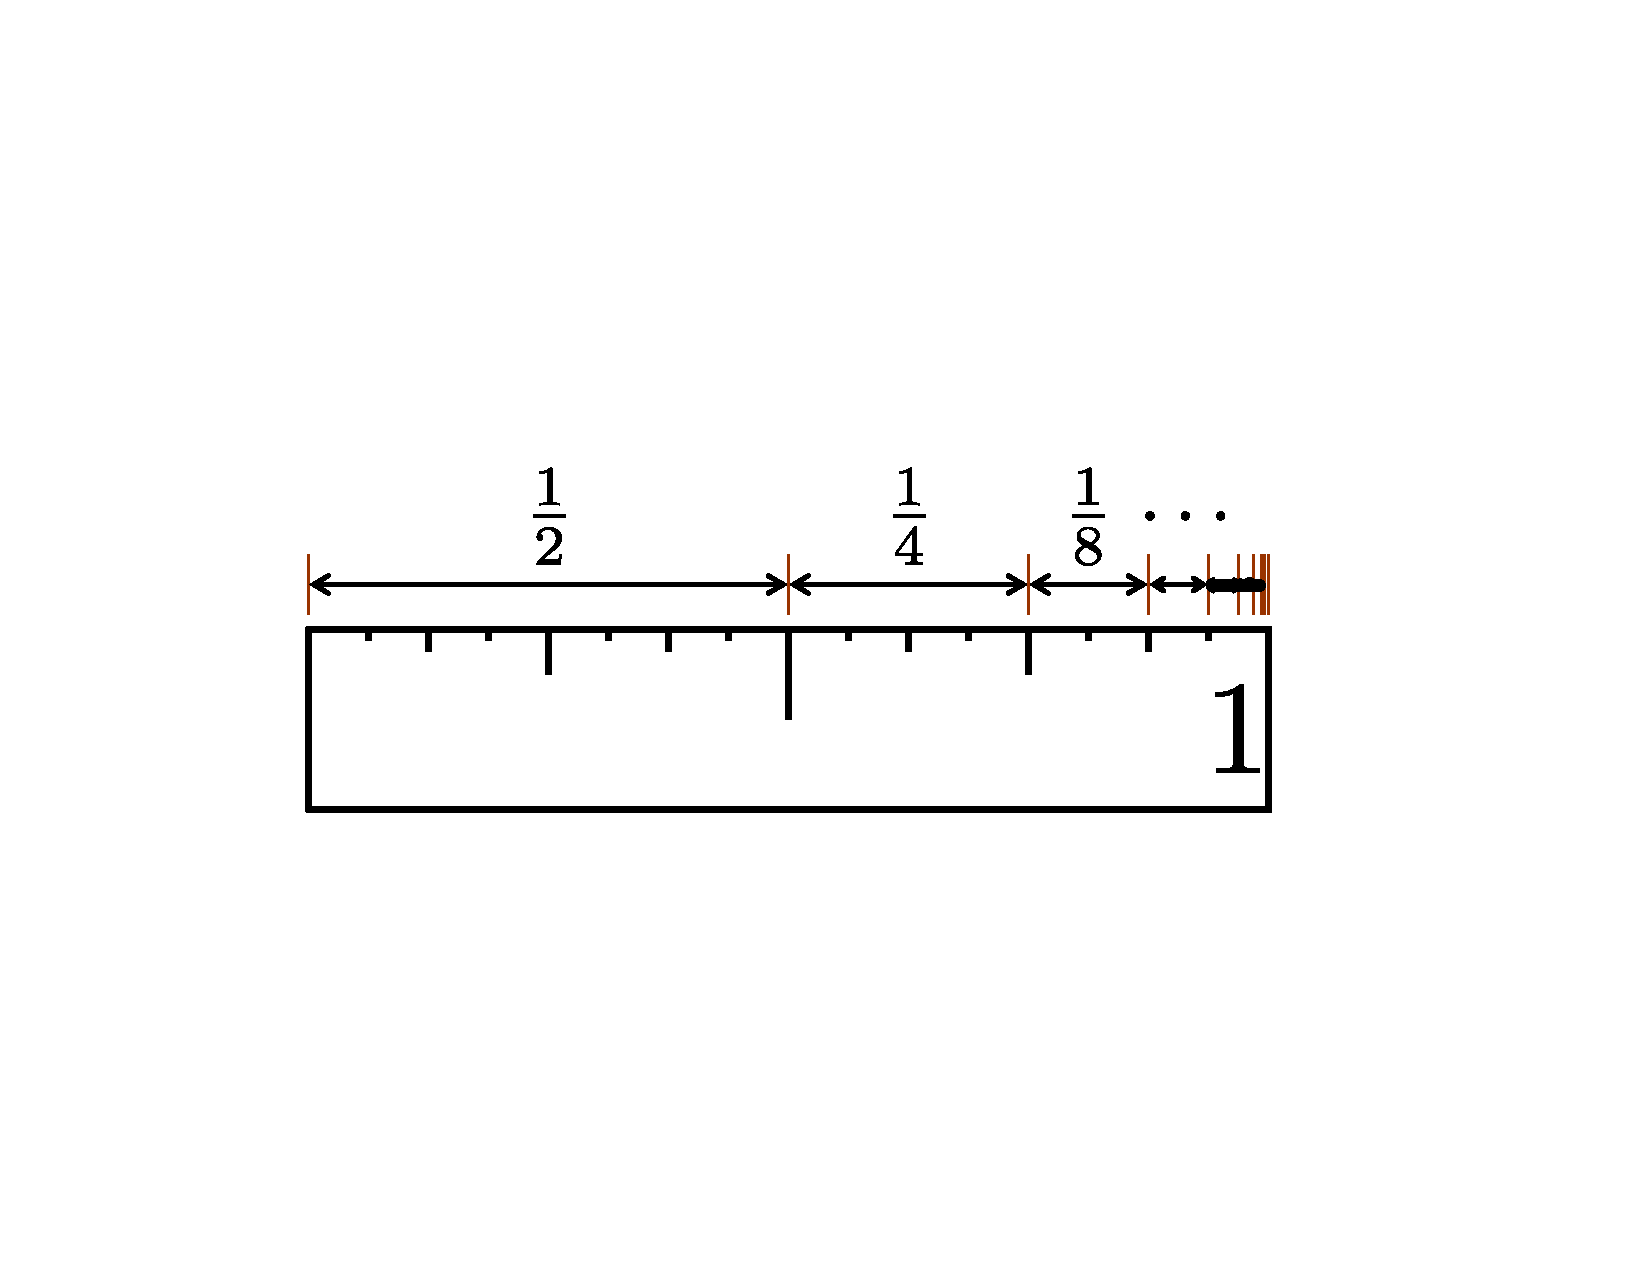
\includegraphics[width=5cm]{pic/GeometricSegment.pdf}
%\end{center}
%\end{figure}
%
%However if we look at the distance traveled after $k$ iterations, we
%get a geometric sum with ratio $\frac{1}{2}$:
%\[
%\frac{1}{2}+\frac{1}{4}
%+\frac{1}{8}+\frac{1}{16}+\cdots+\frac{1}{2^k}
%\]
%If the process continues infinitely many times, we thus get get the
%following formula for the distance traveled:
%\[
%\frac{1}{2} + \frac{1}{4} + \frac{1}{8} + \ldots + \frac{1}{2^{n}} +
%\ldots = \sum_{n=1}^{\infty} \frac{1}{2^{n}}
%\]
%We will see that this sums up to $1$ (i.e. the full distance is traveled,
%resolving the paradox).

%Notice that there is a slight shift in this formula from the one
%given in the definition of a geometric series in that we start not
%with $r^0=1$ but with $r^{1}=\frac{1}{2}$ while in the definition
%this power is zero.  This can be fixed by letting the constant a be
%$\frac{1}{2}$, This sort of index change arises often enough that we
%will first look at how we can manipulate such infinite sums.
%
%\section*{Reindexing a Series}
%We begin this discussion with a brief reminder about the $\Sigma$ notation
%for sums.
%Given $\displaystyle{\sum_{n=1}^{k} a_{n}}$ we call n the
%\textbf{index of summation}, $a_{n}$ the \textbf{$n^{th}$ term} of
%the sum, and the \textbf{upper and lower bounds of summation} are k
%and 1
%respectively.  \\
%
%Now we consider reindexing our infinite series, notice in the
%following examples we are working with geometric series, however
%this algorithm will be useful with other
%types of series that will be discussed later. \\
%
%Most of the infinite series we have seen so far have a lower bound
%of summation of one, however their are times when we are given an
%infinite series where the lower bound of summation will be a value
%other than one. We consider first a geometric series which does not
%have a lower bound of one: $$ \frac{-1}{27} + \frac{1}{81} -
%\frac{1}{243} + \ldots + (\frac{-1}{3})^{n-1} + \ldots =
%\sum_{n=4}^{\infty} (\frac{-1}{3})^{n-1} $$ This is still a
%geometric series, however our definition requires the series to have
%the form $\displaystyle{\sum_{n=1}^{\infty} ar^{n-1}}$, so
%reindexing is required. To re-index a series we follow the following
%basic algorithm:
%\begin{Algorithm}[Re-indexing a series]\ 
%\begin{itemize}
%%\item[1] Choose a new letter to be the index of summation (m)
%\item[2] Relate m to the original index of summation (n) such that when
%n=4 we have m=1.  So we have the equation m=n-3.
%\item[3] Solve for original index of summation (n) and substitute into
%the $n^{th}$ term of the sum: $$ n=m+3 \Rightarrow
%\sum_{m=1}^{\infty} (\frac{-1}{3})^{m+3-1} = \sum_{m=1}^{\infty}
%(\frac{-1}{3})^{m+2} $$ Notice if the upper bound of summation were
%finite we would have to decrease its value by 3 as well, however
%since we are summing to infinity our upper bound of summation will
%remain infinite.
%\item[4] Solve for an a such that the power on r is m-1. $$
%\sum_{m=1}^{\infty} (\frac{-1}{3})^{m+2} = \sum_{m=1}^{\infty}
%(\frac{-1}{3})^{3} \cdot (\frac{-1}{3})^{m-1}$$ since m-1+3=m+2.
%\end{itemize}
%\end{Algorithm}
%Therefore $a=(\frac{-1}{3})^3 = \frac{-1}{27}$ and $r=\frac{-1}{3}$
%so we have a geometric series of the form
%$\displaystyle{\sum_{m=1}^{\infty} ar^{m-1}}$.  Notice that in this
%example the ratio was negative, therefore a geometric series can
%have negative or positive r values. We now look at another example
%of this re-indexing algorithm before we develop an equation for the
%value of a geometric series.
%
%\begin{Example}
%Consider the series $\displaystyle{\sum_{n=9}^{\infty}
%\frac{4}{2n+3}} $, rewrite
%this series so that the lower bound of summation is n=1.
%
%\solution
%Let $m=n-8$, then $n=m+8$ so we have
%$\displaystyle{\sum_{m=1}^{\infty} \frac{4}{2(m+8)+3} =
%\sum_{n=1}^{\infty} \frac{4}{2m+19}}$
%\end{Example}
%
%Using this algorithm we can always manipulate a given geometric
%series so that it can be written in the form
%$\displaystyle{\sum_{n=1}^{\infty} ar^{n-1}}$ or equivalently
%$\displaystyle{\sum_{n=0}^{\infty} ar^n}$ next we consider how to
%calculate the value of this series.
%
%\subsection*{The Formula for the Geometric Series}
%In this section we will derive a general formula for the value of
%$\displaystyle{ \sum_{n=0}^{k} ar^{n}}$. We can apply this in the
%%limit case $k=\infty$ to get the value of an infinite series, for
%example to show that the series $\displaystyle{\sum_{n=1}^{\infty}
%\frac{1}{2^n}}$ from Zeno's paradox has value $1$.

Now consider
\[
p_{k}=a + ar + ar^{2} + \ldots + ar^k
\]
and
\[
rp_{k} = ar + ar^{2} + ar^{3} + \ldots + ar^{k+1}.
\]
Notice that these two expressions share several terms in common, in
fact
\[
p_{k}-rp_{k}= (a + ar + ar^{2} + \ldots + ar^k) - (ar +
ar^{2} + ar^{3} + \ldots + ar^{k+1}) = a -ar^{k+1}
\]
Now if we factor both sides of this equation, we get
\[
p_{k}(1-r)=a(1-r^{k+1}).
\]
As
long as $r \neq 1$ we can divide both sides by $(1-r)$ to get
%\begin{center}
%\fbox{\begin{minipage}{3in}
%\Large
\[
p_{k}=\sum_{n=0}^{k}ar^n=a\frac{1-r^{k+1}}{1-r}.
\]
%\end{minipage}}
%\end{center}

(What happens in the case where r=1?
We get $s_{k}= a + a(1) + a(1)^{2} + \ldots + a(1)^{k-1}=ka$.)
\medskip

Before we go on to get a formula for the infinite sum, we see
how the formula for $p_{k}$ might be used on its own:
%\begin{Example}[The magnitude of repeated growth]
Suppose we are given a chess board and place one grain of rice on
the first square, two grains of rice on the second square, four
grains of rice on the third square continuing on so that there are
$2^{n-1}$ grains of rice on the $n^{th}$ square.  How many grains of
rice are on the chess board? (There are $8\cdot 8=64$ squares on a chess
board.) 
%\begin{figure}
% \epsfig{file=Chess-board-walnut.jpg,scale=.8}
%\end{figure}

%\solution
Since there are 64 squares on the chess board (from $0$ to $63$), we want to compute
$p_{63}$.  Our ratio is 2 and $a$ is one, hence we are asked to find
\[
p_{63}=1+2+4+ \ldots +2^{63} =
\frac{1(1-2^{64})}{1-2} = 1.84467 \times 10^{19}
\]
%\end{Example}

A similar calculation underlies the repayment of loans or mortgages:

%\begin{Example}[Paying back a loan]
Suppose we take out a loan of $L$ dollars which is paid back
periodically (typically monthly). The periodic payment is $a$
dollars, the fixed interest rate \textit{per period} is $i$. If
$b_k$ is the loan sum outstanding after $k$ time periods, we have
that
\[
b_{k+1}=b_k\cdot (1+i)-a.
\]
Using $b_0=L$ and setting $r=1+i$, in the first step we have
\[b_{1}=Lr-a\] we then continue on to the next step where we
get
\begin{eqnarray*}
b_{2}&=&b_{1}(r)-a 
=(Lr-a)(r)-a \\
&=&Lr^{2}-(a+ar)
\end{eqnarray*}
We might be starting to notice a pattern, however it becomes obvious
in the next step
\begin{eqnarray*}
b_{3}&=&b_{2}(r)-a 
=(Lr^{2}-(a+ar))(r)-a \\
&=&Lr^{3}-(a+ar+ar^{2})
\end{eqnarray*}
At this point we can solve this recursion to
\[
b_k=L\cdot r^k-\left(a+ar+ar^2+\cdots+ar^{k-1}\right)
=L\cdot r^k-\sum_{n=0}^{k-1}ar^n
\mathop{=}\limits^{\mbox{\quad Sum formula\quad}}L\cdot r^k-a\frac{1-r^k}{1-r}.
\]
A bank now would set $b_m=0$ (where $m$ is the time after which the loan
should be paid off, e.g. $m=12\cdot 30=360$ for a 30 year mortgage)
and solve for $a$ to determine the
necessary monthly repayment, given the loan sum and interest rate.

For example, if we have a mortgage of $L=\$200,000$, an annual
interest rate of $6$\% (leading to a monthly rate of
$i=.06/12=0.005$, i.e. $r=1.005$) and a monthly repayment
sum\footnote{Slightly moralistic remark: Incidentally, initial interest amounts
to {\$}$1000$ per month at the start of the loan. An
\textit{interest only} loan thus does not save much and is a very
bad deal!} of $a=\$1,200$, we find that the outstanding sum after
$k$ months is
\[
b_k=200,000\cdot{1.005^k}-1,200\frac{1.005^k-1}{0.005}
=200,000\cdot{1.005^k}-240,000\left(1.005^k-1\right).
\]
After $10$ years ($120$ months) this leaves an outstanding amount of
{\$}$167,224.13$, after $20$ years {\$}$107,591.82$, roughly
half\footnote{In general, this means that a loan is paid off half
after roughly $\frac{2}{3}$ of its planned life time}, after $30$
years {\$}$-903.00$ (i.e. the loan is paid off after $30$ years less
one month\footnote{The total cost of the loan then will have been
{\$}$430,800$, more than double the loan amount. (Though inflation
means that the actual value will be less.)}).

If the interest rate instead was $7$\% annually ($i=.07/12=0.005833$
monthly), we get with same repayment sum a remaining loan amount of
{\$}$159,256.18$ after $30$ years, which is not even halfway paid
off. A monthly repayment sum of {\$}$1330$ would be
needed\footnote{I.e. a change of one percentage point in the
interest rate increased the monthly payment (and thus the total loan
cost) by $10$\%! No wonder people go bonkers about interest rates.}
to have the loan paid off after $30$ years.
%\end{Example}
\medskip

Since the sequence $p_0, p_{1}, p_{2}, 
\ldots, s_{k}, \ldots$ of partial sums converges to
$\displaystyle{\sum_{n=1}^{\infty} ar^{n-1}}$, we can use the
formula just derived to compute a value for the limit of a geometric series:

If $\sz{r}<1$, we have that $\lim_{k\to\infty} r^{k+1}=0$ and thus

\[
\sum_{i=0}^{\infty} ar^i
=
\lim_{k\to\infty} p_k=
\lim_{k \rightarrow \infty} \frac{a (1-r^{k+1})}{1-r} =
\frac{a(1-0)}{1-r}=\frac{a}{1-r}.
\]
This incidentally verifies the above example
\[
\sum_{i=0}^\infty \frac{1}{2^i}=2
\]

On the other hand, if $\sz{r}\ge 1$, the absolute value of the numerator
$1-r^{k+1}$ will go towards infinity, and the series diverges.


%\begin{center}
%\fbox{\begin{minipage}{\textwidth}
%\begin{Theorem}
%The geometric series $\displaystyle a + ar + ar^{2}+ \ldots +
%ar^{n-1} + \ldots =\sum_{n=1}^{\infty} ar^{n-1}$ converges to
%$\displaystyle\frac{a}{1-r}$ when $|r|<1$, and diverges otherwise.
%\end{Theorem}
%\end{minipage}}
%\end{center}
%\begin{proof}
%\textbf{Case 1:} If $|r|<1$ then $|r|^{k} <1$, and as $k$ gets
%larger this will cause $|r^{k}|$ to get smaller and yield
%$\displaystyle\lim_{k \rightarrow \infty} r^{k}=0$. Thus, by the rules for
%limits,
%
%\\
%\textbf{Case 2:} When $|r| \geq 1$ then $|r|^{k} \geq
%1$. Therefore when $k$ tends to infinity the numerator $a(1-r^{k})$
%tends to plus or minus infinity, and the denominator $1-r$ is a fixed
%value. So $\displaystyle{\lim_{k \rightarrow \infty}
%\frac{a
%(1-r^{k})}{1-r}}$ diverges.
%\end{proof}
%
%Now that we have a formula for the value of a geometric series let
%us verify the solution to the Zeno's paradox example.  We are
%looking at $\displaystyle{\sum_{n=1}^{\infty}\frac{1}{2^n}}$. First
%notice that this sum is not in the correct form,  we must factor
%$(\frac{1}{2})$ out of the $n^{th}$ term.  We get
%$\displaystyle{\sum_{n=1}^{\infty} ( \frac{1}{2})^{n} =
%\sum_{n=1}^{\infty}(\frac{1}{2})\cdot(\frac{1}{2})^{n-1}
%=\sum_{n=0}^{\infty} (\frac{1}{2}) \cdot (\frac{1}{2})^{n}}$, hence
%$a=\frac{1}{2}$ and $r=\frac{1}{2} < 1$ so this series converges to
%\[
%\frac{a}{1-r} =
%\frac{\frac{1}{2}}{1-\frac{1}{2}}=\frac{\frac{1}{2}}{\frac{1}{2}}=1.
%\]

%Next we will look at some interesting examples where we can use this
%formula.
%
%\section*{Examples}
%In this section we will look at how people may use geometric series
%in real life applications.
%
%In our first example we
%look at how much
%medication will remain in a persons body after taking medication at
%regular intervals
%\begin{Example}[Repeated Drug Dosage]
%A CSU student comes down with bacterial laryngitis, the student goes
%to the Healthcenter to see a doctor who prescribes 250mg doses of
%antibiotics that the student must take every six hours over the next
%several days.  Since the body will digest the antibiotics between
%doses and it is known that 5 percent of the drug remains in the body
%at the end of six hours, how can we calculate the quantity of the
%drug that remains in the student after the fifth dose? At the end of
%five full days on the drug?
%
%\solution
%Let us begin by looking at the quantity of the drug in the body
%after each dose.  Let $q_{n}$ represent the quantity of the drug in
%the students body after the $n^{th}$ dose.  Initially $$ q_{1}=250$$
%at the next dose we will have 5\% of that 250mg remaining and
%another 250mg is taken, so $$q_{2}=250(0.05)+250$$ At the third dose
%we have 5\% of $q_{2}$ remaining and another 250mg is taken, so
%therefore
%\begin{eqnarray*}
%q_{3}&=&0.05 \cdot q_{2} +250 =0.05(250(0.05)+250) +250\\
%&=&250(0.05)^{2} + 250(0.05) + 250.
%\end{eqnarray*}
%Now on the fourth dose
%$q_{4}$ we have $0.05 \cdot q_{3}$ remaining in the body and another
%250mg is taken.
%\begin{eqnarray*}
%q_{4}&=&0.05 \cdot q_{3} + 250
%=0.05(250(0.05)^{2} + 250(0.05) + 250) + 250\\
%&=&250(0.05)^{3} + 250(0.05)^{2} + 250(0.05) + 250.
%\end{eqnarray*}
%Notice at this point that a
%pattern has developed, we have $$q_{n}=s_{n}=\sum_{k=1}^{n}
%250(0.05)^{n-1}$$ Therefore we can use our formula
%%$s_{n}=\frac{a(1-r^{n})}{1-r}$ to calculate
%$q_{n}=\frac{250(1-0.05^{n})}{1-0.05}$.  With this information we
%can calculate $q_{5}=\frac{250(1-0.05^{5})}{1-0.05} = 263.1578125$mg
%in the students body after 5 doses.  If the student continues to
%take the antibiotic for 5 full days or 20 doses they will have
%$q_{20}=\frac{250(1-0.05^{20})}{1-0.05}=263.1578947$mg. \\
%
%Suppose the student continued to take this drug forever, how much
%medication would there be in the students body at each dose?\\
%
%This question is asking us to compute
%$\displaystyle{\sum_{n=1}^{\infty} 250(0.05)^{n-1}}$ which luckily
%for the student $0.05<1$ will converge to a finite number of
%$\frac{250}{1-0.05}=263.1578947$mg. Since $0.05^{20}=9.536743 x
%10^{-27}$ which is practically zero, we get the same value up to the
%ten-millionth place if the student took the medication forever as we
%got when the student took the medication for five days.
%
%\end{Example}
%
%\begin{Example}[Repeating Decimal]

As an example application of this formula, we look at how one can
express the repeating decimal $0.\overline{08}$ as a fraction of two integers.

%\solution
%To express $0.\overline{08}$ as a fraction 
We first notice that $08$
is the repeated value, so we want to break up $0.\overline{08}$ into
a sum of the repeated values.  Therefore we have $0.\overline{08}=
0.\underline{08}+ 0.00\underline{08}+ 0.0000\underline{08}+ \ldots$.
Once we have this written as a sum we can now write each term in the
sum as a fraction, hence we have $0.\underline{08}=\frac{8}{100}$,
$0.00\underline{08}=\frac{8}{10,000}=\frac{8}{100^{2}}$, and
$0.0000\underline{08}=\frac{8}{100^{3}}$.  Using this information we
should recognize a pattern $$0.\overline{08} = \frac{8}{100} +
\frac{8}{100^{2}} + \frac{8}{100^{3}} + \ldots = \sum_{i=1}^{\infty}
\frac{8}{100^{i}}$$ However at this point we notice that we have a
geometric series which is not written in the correct form for us to
apply our formula.  If we factor out $(\frac{8}{100})$ we get
$\displaystyle{\sum_{i=0}^{\infty}
(\frac{8}{100})(\frac{1}{100})^i}$ which is now in the correct
form. This gives $r=\frac{1}{100} <1$ so our geometric series
converges and since $a=\frac{8}{100}$ the series converges to
$$\frac{\frac{8}{100}}{1-\frac{1}{100}}=\frac{\frac{8}{100}}{\frac{99}{100}}=\frac{8}{99}=0.\overline{08}.$$
%Being able to express a repeating decimal as a fraction is useful
%when we are calculating with a large number of values where the
%precision of the answer is vital since a fraction will not have
%any round off error.  \\
%\end{Example}

For another example, consider the following paradox of Zeno\footnote{Zeno
of Elea, Greek philosopher, ca. 490 BC - ca. 430 BC}:

Achilles, the fastest runner in ancient Greece, runs 100 times as
fast as the Tortoise. But --- so the paradox claims --- if the
Tortoise is given an advance, Achilles will never be able to pass
the Tortoise:

%\begin{Example}[Achilles and the Tortoise]
Suppose that Achilles runs
$10 m/s$ and the Tortoise only $0.1 m/s$, furthermore the Tortoise is given
a head start of $100m$.
After $10$ seconds, Achilles has reached the place where the Tortoise
started. But in this time, the Tortoise has run $1m$ ahead. Achilles will
reach this distance in $0.1$ seconds. But then the Tortoise has moved
another $0.01m$. Achilles will take $0.001$ seconds to reach this, and so
on. He will never reach the Tortoise. Where is the error in this argument?

%\solution
The paradox is resolved, if we realize what time period is considered:
All events take place within
\[
10+0.1+0.001+\cdots=10\sum_{n=0}^\infty
\frac{1}{100^n}=\frac{10}{1-\frac{1}{100}}=\frac{1000}{99}=10.\overline{10}
\]
seconds. This is exactly the time {\em when Achilles reaches (and
overtakes!) the Tortoise}. The paradox arises from the implicit
(and wrong, as we have calculated!)
suggestion, that it describes the events for all time.
%\end{Example}

\section{Arithmetic Series}

While not directly related to the Geometric Series, this seems to be an
appropriate place to also look at summations over other sequences.

The summation over a constant sequence with fixed value $a$,
\[
\underbrace{a+a+\cdots +a}_{\mbox{$n$ terms}}=n\cdot a
\]
is basically just the definition of multiplication. But what happens if the
terms change by a constant sum, that is we have that $a_{i+1}-a_i=c$
constant.

Let us first observe this for the basic case of 
\[
S_n=\sum_{i=1}^n i=1+2+\cdots+n.
\]
We get a formula by writing this sum down a second time in reversed order
and add both up (thus getting {\em twice} the value $S_n$):
\[
\begin{array}{ccccccc}
&1&+2&+3&+\cdots&+(n-1)&+n\\
+&n&+(n-1)&+(n-2)&+\cdots&+2&+1\\
\end{array}
\]
We can get the value in another way by first adding down in each column.
Note that each column adds up to $n+1$, and we have $n$ columns, and this
sum thus is $n(n+1)$. This gives us the formula:
\[
\sum_{i=1}^n i=1+2+\cdots+n=\frac{n(n+1)}{2}.
\]
For example, we get that
\[
1+2+\cdots+100=\frac{100\cdot 101}{2}=\frac{10100}{2}=5050.
\]
If subsequent terms differ by a different constant, we can handle this with
a factor (and possibly a starting term. Suppose we start at 5 and differ by
3 in each step:
\[
5+8+11+14+\cdots+32
\]
we subtract $2$ from each summand, so that they all are a multiple of $3$,
and then separate the two operations:
\[
=(2+3)+(2+6)+(2+9)+\cdots(2+30)=\underbrace{2+\cdots+2}_{\mbox{$10$ terms}}
+3\left(1+2+\cdots+10\right)
\]
We know that there are 10 terms, as we have $(32-5)/3=9$ steps from the
first. Now we use the two kinds of formulas and get
\[
5+8+11+14+\cdots+32=10\cdot 2+ 3\cdot\left(\frac{10\cdot
11}{2}\right)=20+3\cdot 55=185.
\]
We note, without proof, the similar formulas:
\begin{eqnarray*}
\sum_{i=1}^n i^2&=&\frac{n(n+1)(2n+1)}{6}\\
\sum_{i=1}^n i^3&=&\frac{n^2(n+1)^2}{4}\\
\end{eqnarray*}

%\subsection{Other Sums}
%
%there is a constant factor $a$, such that
%every term is the $a$-times multiple of the previous term. That is
%
%The partial sums over this sequence are thus
%\[
%\sum_{j=0}^i a^i r = r\cdot\sum_{j=0}^i a^i
%\]
%Multiplying this expression by $1-a$ gives us
%\begin{eqnarray*}
%(1-a)(r\sum_{j=0}^i a^j)&=&r\left(\sum_{j=0}^i a^j-a\sum_{j=0}^i a^j\right)\\
%&=&r\left(\sum_{j=0}^i a^j-\sum_{j=1}^{i+1} a^j\right)=r\left(a^0-a^{i+1}\right)
%=r\left(1-a^{i+1}\right)
%\end{eqnarray*}
%and (dividing again by $1-a$)
%\[
%\sum_{j=0}^i ra^i=r\frac{1-a^{i+1}}{1-a}
%\]
%This formula is called the summation formula for the geometric series and has many
%practical applications.

